% vim:ft=tex
\documentclass[a4paper,11pt]{scrartcl}
\usepackage{tohojo-xe}
%\selectlanguage{english}
\setcounter{secnumdepth}{1}
\setcounter{tocdepth}{2}
\hypersetup{pdfauthor={Toke Høiland-Jørgensen, Mikkel Hartmann, Dan 
Albrechtsen, Malik Thrane, Troels Christensen, Wence Xiao}, pdftitle={Crowd 
modeling}}

\title{Crowd modeling}
\author{Toke Høiland-Jørgensen, Mikkel Hartmann, Dan Albrechtsen, Malik 
Thrane, Troels Christensen, Wence Xiao}
\date{2010-09-12}
\fancyhead[OR,EL]{\footnotesize Draft: \timestamp}
%\type{}
 
 
\begin{document}

\begin{titlepage}
    \begin{center}
		\begin{sf}
            {\Huge \textsc{\textbf{Crowd modelling\\[2cm]
            }}} Picture here %\includegraphics[width=15cm]{figurer/forside}
            \\[2cm]

            {\large Toke Høiland-Jørgensen \\
            Mikkel Hartmann\\
            Dan Albrechtsen\\
            Malik Thrane\\
            Troels Christensen\\
            Wence Xiao\\
            [0.5cm] }

            {\small \textbf{Advisor}\\
            Viggo Andreasen}
			\vfill
            Modeling project, fall 2010\\
            Mathematics RUC
		\end{sf}
	\end{center}

    \clearpage
%    % vim:ft=tex

\begin{abstract}
    \section*{Abstract}
    \small
    We look at social force models as a way to model the behaviour of human 
    crowds, in order to evaluate what these types of models can tell us about 
    crowds, which assumptions underlie them and what their strengths and 
    weaknesses are. In order to do this evaluation, we implement a computer 
    simulation of an exemplary social force model.

    In order to create this simulation, we pick an exemplary model that is 
    described in detail in the article that presents it, and analyse it in 
    detail, filling in details from other articles where necessary. Based on 
    this analysis of the model, we go from the abstract model formulation to a 
    concrete numerical simulation by filling in required details, such as  how 
    to approximate the movement of pedestrians, how to set initial conditions 
    and values, and how to implement the interaction between pedestrians and 
    walls in practice.

    From our results, it is clear that our simulation (with the right 
    parameters) exhibits reasonable pedestrian behaviour upon visual 
    inspection. While we successfully replicate some results from the 
    literature, other effects do not manifest themselves. We discuss several 
    reasons for this discrepancy, including features that are lagging from the 
    model, parameter values, effects of using random numbers to generate the 
    initial conditions and possible errors in our implementation of the model.

    Based on the results of our own simulations and our review of the social 
    force modelling field, we assess social force models and their strengths 
    and weaknesses. We conclude that social force models are not built on any 
    theories for the behaviour of crowds, but are created to replicate a set 
    of observations. As such, any confidence in their predictions must come 
    from a record of producing results fitting observations; and since the 
    field is relatively new, they have not yet reached this state. Social 
    force models do, however, provide a practical way to simulate something 
    that would otherwise be impossible to simulate. As such, they are the best 
    available way to provide e.g. guidance when designing facilities that must 
    accommodate many pedestrians, and given time the accuracy of their 
    predictions will probably increase.
\end{abstract}
\begin{abstract}
    \section*{Resume}
    \small
\end{abstract}

\end{titlepage}

\tableofcontents
\listoffigures

\clearpage

% vim:ft=tex
\section{Introduction}
When a lot of people are gathered in a confined space, it is not immediately 
obvious how they behave when moving around. It is also not obvious how to 
design buildings and other areas where many people gather to allow for optimal 
passage of crowds without jamming and related problems (such as inconvenience 
for pedestrians and even injuries). It is cumbersome, or even dangerous, to 
gather many people together to do experiments, especially if one wishes to 
simulate a panic situation (which cannot necessarily be induced artificially).  
It would thus be useful to be able to model a crowd of pedestrians and their 
movement.

A crowd of many people is a very complex system. One of the approaches to 
handling this complexity is by using a computer simulation of a model derived 
from the behaviour of individual pedestrians, and through the outcome of this 
simulation be able to say something meaningful about the whole system. This 
approach to modelling complex systems is called agent-based modelling and is 
used in many different and diverse subject areas, including molecular biology, 
economics and physics.

Within the field of crowd simulations, there  are various ways of formulating 
such an agent-based model; we have chosen to focus on an approach that models 
pedestrian behaviour using a concept called ``social forces'' 
\cite{social-force}. This type of model describes individual behaviour 
borrowing concepts and notation from physics, by defining  virtual ``forces'' 
representing desired movement as well as the tendency to avoid obstacles, 
other people etc. Through computer simulations this can be used to say 
something about the whole system of moving pedestrians.

Since the original formulation of the social force concept, it has been 
revised several times (e.g.  \cite{helbing00}). For this project we base our 
analysis on the  version presented in \cite{self-org}, as this article goes 
into a reasonable level of detail. We will, however, also include other 
variants where necessary.  Our chosen model, and others like it, describe a 
set of properties of crowd behaviour that has been seen in observations of 
actual crowds as well as replicated in computer simulations.  We think it will 
be interesting to go into detail with this type of model and look into how 
they work and what they can tell us about crowds. This brings us to our 
problem formulation:

\subsection{Problem formulation}
\begin{quote}
    How do social force models work and what do they say about crowds?

    What are the assumptions underlying social force models, and what are 
    their strengths and limitations?
\end{quote}

Our problem is exemplary to mathematical modelling for several reasons. First 
of all, it is an example of applying mathematical theory to a field outside of 
mathematics itself. The field we are working with (crowd simulation) is 
relatively new, but has some established research\footnote{See the overview of 
the field in section~\ref{sec:social-forces}.}. The model itself contains a 
non-trivial application of mathematics and is an example of a type of model 
(agent-based models) used in many cases to study a complex system of 
interacting pedestrians by describing the individual behaviour of the pedestrians and 
using simulations to derive meaningful properties for the whole system. These 
factors combined makes our problem exemplary.
% TODO: References for agent-based models.

\subsection{Target audience}
The target audience of this report is comprised of students of mathematics on 
a level of education similar to our own. This means that we consider 
mathematical concepts and theory that is covered in the bachelor courses at 
the mathematics department at RUC as known subject matter, and will therefore 
not explain these concepts in detail. Concepts that are beyond this are 
explained as necessary. In the description of the simulation program code, 
some familiarity with basic constructs of computer programming is assumed, and 
are thus not explained.

\subsection{Approach to answering the problem formulation}
To answer the problem formulation, it is first necessary to establish the 
concept of social force models in more detail, as well as give an overview 
over the work in the field. This is presented in 
section~\ref{sec:social-forces}, where we also present the model we have chosen 
to focus on, including the results presented in it.

In order to better understand the model, we are going to make our own computer 
simulation of it. To do so, we will first describe the model thoroughly. In 
section~\ref{sec:the-model}, we will go over the different parts and 
parameters of the model, and point out parts that are ambiguous or missing 
from the article presenting the model.  Based on this description, we will 
discuss what is needed to turn the model into a numerical simulation, and how 
we have done so, in section~\ref{sec:model-to-simulation}.

Based on our analysis of the model, we will construct a computer simulation of 
it, modelling cases analogous to those presented in 
section~\ref{sec:social-forces}. Our implementation of the 
simulation is discussed in section~\ref{sec:simulation}, including set up of 
parameters and initial conditions, the structure of our simulation and how we 
obtain results from it.

The actual results of the simulation is addressed in 
section~\ref{sec:results}. Here we present the outcome of our simulation, and 
whether or not we have been able to replicate the results we were aiming for.  
Based on this presentation, we discuss in section~\ref{sec:discussion} 
possible reasons for any discrepancies between our own results and the results 
we are trying to replicate, as well as which alterations of the model would 
be needed to fix them.

Based on our results and the proposed changes to the model, we will assess 
social force models in general in section~\ref{sec:assessment}, giving an 
overview of the strengths and weaknesses of this modelling approach. Finally, 
we will give a summary of our findings and an overview of the whole project in 
section~\ref{sec:conclusion}.

\clearpage
% vim:ft=tex
\section{Analysis of the model}
\subsection{Social force models}
The idea behind social force models is that each individual in the crowd acts on his/ her own from a personal aim or goal and by behavioral reactions to
the environment. Different forces such as other pedestrians, walls and obstacles are taken into account when pedestrian $\alpha$ walks toward his/her aim or
goal, so that $\alpha$ does not walk into another pedestrian or wall. The forces influencing the pedestrian $\alpha$'s motion of direction are not forces
acting on $\alpha$'s body, but has to be seen as a quantity that describes the motivation to act.
Since pedestrian $\alpha$ is used to the situations he/she is normally confronted with, his/her reactions will be rather automatic and determined by his/her
experience of which reaction will be that best. Since the reaction is rather automatic it is possible to put the rules of pedestrian behavior into an
equation of motion. [Helbing and Molnár, 1995]

There are other ways to model crowd than social force models such as Rule Based models, Cellular Automata models and HiDAC. Below we will make a short
explanation of each of the other crowd models.
\\

\textbf{Rule Based models}\\
Rule Based models describe the movement of pedestrians through sets of basic rules. Each pedestrian apply collision detection and avoidance to prevent
collision with other pedestrians. However they do not in general apply collision response, and therefore collisions and overlappping of the pedestrians
may occur under some circumstances. Some models have applied stopping rules to prevent these situations. [Pelechano et al., 2008]

\textbf{Cellular Autamata models}\\
These models are discrete, deterministic and is made up of cells like the squares in a chessboard.
An artificial intelligence approach is used in Celluar Automata (CA) defined as mathematical idealisation of physical systems in which time and space are
discrete, and physical quantities take a finite set of discrete values. Pedestrian can not collide since the floor is dicretised and the pedestrians can
only move to free adjecent cells. [Pelechano et al., 2008]

\textbf{HiDAC}\\
The HiDAC model is made as a hybrid between social force models and rule based models. The motion of the pedestrians is caried out like the social force
models, but is also based on the psychological and geometrical rules. It peforms collision detection and response and rules are applied depending on the
pedestrian's personality and the state of the environment. [Pelechano et al., 2008]
\\
\\

\textbf{Geometrical features of the models}\\
Each of the different models have some geomatrical features relatively important and unimportant according to our simulation.

\textbf{Shaking} Wether pedestrians appear to shake when simulating the model.
When simulating the social force models the pedestrians seems to shake when cloggings and queues arise. This is caused by the modification
of each pedestrians postition in each timestep. 
The HiDAC, CA and rule based model do not appear to shake while the simulation run.

\textbf{Discrete and Continuous movement} Wether the space and time are discretised. In the CA model the pedestrians move between discritised adjecent
cells in one time step, and therefore have limited direction to go. The other models do not discretise space and therefore allow the pedestrians to move
within continuous space.
 
\textbf{Overlapping} Wether overlapping of the pedestrians is possible. The rule based models and the CA models do have collision detection but not
all have collision responce. The CA models have rules so that a pedestrian can not walk into an occupied cell, but if two pedestrians want to pass each
other they step into the cell diagonal to their own cell, and in their way cross the other pedestrian in the intersection between the four cells.
Newer models of the rule based and CA have made a stopping rule so that overlapping can not accour. The HiDAC and social force models do collision responce
to minize the risk of overlapping. [Pelechano et al., 2008]

\textbf{Pushing} Wether pedestrians can have physical contact. If the pedestrians can have physical contact they will be able to push each other in some
direction. This ability is possible when using the HiDAC and the social force model. When simulating evacuations and chaotic events it has been observed
that people do have physical contact and push each other [Helbing et at., 2005].

\textbf{Communication} Wether the pedestrians can share information about he environment. The HiDAC and som newer rule based models allows the pedestrians
to share information about the environment and to give orders. This feature is not included in social force models and CA. [Pelechano et al., 2008]

To illustrate different features of the different models the table below sums up the above mentioned.
\begin{center}
\begin{tabular}{lllll}
 & Social Forces & Rule Based & CA & HiDAC\\
Shaking avoidance     & - & + & + & +\\
Continuous space      & + & + & - & +\\
Overlapping avoidance & + & * & - & +\\
Pushing               & + & - & - & +\\
Communication         & - & * & - & +
\end{tabular}
\end{center}
Here ``+`` indicates that the feature is possible, ``-`` indicates it is not, and ''*'' that the model has been adjusted such that the feature have
become possible. [Pelechano et al., 2008]

The features we are interested in and find relevant in our simulation are continuous space, pushing and overlapping avoidance. The continuous space is
relevant for our simulaion to be as realistic as possible since we do not want our pedestrians to have at most nine directions to go each timestep.
The feature of pushing is also important to include since in panic sitiation it has been seen that people push each. This feature will then make our
simulation more realistic.
The overlapping avoidance we find relevant since this enables pedestrians to walk through each other.

\clearpage

\subsection{Explanation of the model}
In this section we will go through the model from the article \cite{self-org} in great detail. 
First of all,  as stated briefly earlier this model is an agent based social force model. 
This means that the model uses individual entities to say something about the crowd as a whole. 
Each entity or agent is acted on by a collection of different forces. These forces can be
either repulsive or attractive. The general approach of the model is fairly simple. An agent
$\alpha$ wants to go in a desired direction with a desired speed. However the environment 
and other agents might force agent $\alpha$ to stray from the desired direction or have speeds 
different from the desired one. The change in position of agent $\alpha$ is given by:

	\begin{equation}
		\frac{d \vec{r_{\alpha}}}{dt} = \vec{V_{\alpha}} \left( t \right)
	\end{equation}

And, as we know from newtonian physics, the acceleration of agent $\alpha$ is 
then given by the summation of all the forces acting on the agent:

\begin{equation}
    \frac{d \vec{V_{\alpha}}}{dt} = \vec{f_{\alpha}} \left( t \right) + 
    \vec{\xi_{\alpha}}\left( t \right)
\end{equation}

here $\vec{\xi_{\alpha}} \left( t \right)$ is a random fluctuation of agent $\alpha$. This
force is there to incorporate the fact that fact the identical initial condition
generally will not lead to the same series of events. $\vec{f_{\alpha}} \left( t \right)$ 
is a summation of all the forces action in agent $\alpha$ from the environment 
and other agents. More specifically it is given by:

\begin{equation}\label{model}
    \vec{f_{\alpha}} = \vec{f^{0}_{\alpha}}\left( \vec{V_{\alpha}} \right) + 
    \vec{f_{\alpha B}} \left( \vec{r_{\alpha}} \right) +
    \sum_{\beta \neq \alpha} \vec{f_{\alpha \beta}} \left(\vec{r_{\alpha}}, 
    \vec{V_{\alpha}}, \vec{r_{\beta}}, \vec{V_{\beta}} \right) +
    \sum_{i} \vec{f_{\alpha i}} \left( \vec{r_{\alpha}}, \vec{r_{i}}, t 
    \right)
\end{equation}

So this is a summation of four different kinds of forces. We will go through 
them one at a time explaining their role in the model and their mathematical 
structure. The first term on the right hand side is a velocity dependent force 
and it is given by:

\begin{equation}
	\vec{f^{0}_{\alpha}}\left( \vec{V_{\alpha}} \right) =
    \frac{1}{\tau}
    \left( V_{\alpha}^{0} \vec{e_{\alpha}} - \vec{V_{\alpha}} \right)
\end{equation}

Here $\tau$ is the relaxation time. $\vec{V_{\alpha}}$ is the 
current velocity of the agent and $V_{\alpha}^{0}$ is the initial speed, that is 
the speed of the agent at the end of the last simulation step. $V_{\alpha}^{0}$ is given by:

\begin{equation}
    V_{\alpha}^{0} = \left[ 1 - \eta_{\alpha} \left( t \right) \right] 
    V_{\alpha}^{0} \left( 0 \right) +
    \eta_{\alpha} \left( t \right)V_{\alpha}^{\text{max}}
\end{equation}

Here $V_{\alpha}^{0} \left( 0 \right)$ is the velocity at the beginning of the 
first simulation step and $V_{\alpha}^{\text{max}}$ is the desired speed of agent
$\alpha$, that is the speed that agent $\alpha$ will try to get if it is allowed by the 
environment and other agents. $V_{\alpha}^{\text{max}}$ can be exceeded. $\eta_{\alpha}$ 
is called the impatience or nervousness of the agent and is given by:

\begin{equation}
	\eta_{\alpha} \left( t \right) =
    1 - \frac{\overline{V}_{\alpha} \left( t \right)}
             {V_{\alpha}^{0} \left( t \right)}
\end{equation}

Here $\overline{V}$ is the average speed in the desired direction and as 
earlier $V_{\alpha}^{0} \left( 0 \right)$ is the speed at the beginning of the 
first calculation step of the simulation.

Now the second term on the right hand side of \eqref{model} is the forces acting on agent 
$\alpha$ from the walls of the room. The force is given by:

\begin{equation}
    \vec{f_{\alpha B}} \left( \vec{r_{\alpha}} \right) =
    - \nabla_{\vec{r_{\alpha}}} V_{B}
    \left( \| \vec{r_{\alpha}} - \vec{r_{B}^{\alpha}} \| \right)
\end{equation}

Here $\nabla_{\vec{r_{\alpha}}}$ is the gradient and $V_B$ is a repulsive 
potential. $ \| \vec{r_{\alpha}} - \vec{r_{B}^{\alpha}} \|$ is the distance 
from agent $\alpha$ to the nearest point of the nearest wall.

The repulsive potential describes the force added from the walls to pedestrian $\alpha$, since $\alpha$ does not
want to get too close to the wall. So the closer $\alpha$ get to the wall the more the force from the wall gets.
The repulsion potential is given by  $V_{B} \left( \| \vec{r_{\alpha}} - \vec{r_{B}^{\alpha}} \| \right) =
V^0_{\alpha B} e^{- \| \vec{r_{\alpha}} - \vec{r_{B}^{\alpha}} \| / R }$

Here $V^0_{\alpha B}$ is a constant and $R$ is the radius of a pedestrian.

The reason for this repusion force from the wall is that the pedestrians do not want to get hurt by running into the walls
or get crushed between the panicing crowd and the wall [Helbing and Molnár, 1995].

The third term on the right hand side of \eqref{model} is a summation of all the 
force between agent $\alpha$ and agent $\beta$. It is a function of the position vector and the velocity of 
both agents, and it is given by:

\begin{equation}
    \sum_{\beta \left( \neq \alpha \right)}
        \vec{f_{\alpha \beta }}\left( t \right) =
        A_{\alpha}^{1} exp \left(
            \frac{ r_{\alpha \beta} - d_{\alpha \beta }}
                 {B_{\alpha}^1}
        \right)
    \vec{\eta_{\alpha \beta}} \cdot
    \left(
        \lambda_{\alpha} + \left(
            1 - \lambda_{\alpha}
        \right)
    \right) +
    A_{\alpha}^{2} exp\left(
        \frac{r_{\alpha \beta} - d_{\alpha \beta}}
             {B_{\alpha}^{2}}
    \right)
    \vec{\eta_{\alpha \beta}}
    \label{agentinteraction}
\end{equation}

Here $A_{\alpha}^{1}$, $A_{\alpha}^{2}$, $B_{\alpha}^{1}$, $B_{\alpha}^{2}$ 
and $\lambda_{\alpha}$ are all constants that can differ for each agent. 
$r_{\alpha \beta}$ is the sum of the radii of $\alpha$ and $\beta$ that is 
$r_{\alpha \beta} = r_{\alpha} + r_{\beta}$. $d_{\alpha \beta}$ is the 
distance from the center of mass of agent $\alpha$ and the center of mass of 
agent $\beta$ and is therefore given by $d_{\alpha \beta} = 
\|\vec{X_{\alpha}}\left( t \right) - \vec{X_{\beta}}\left( t \right) \|$. Here 
$\vec{X_{\alpha}}\left( t \right)$ amd $\vec{X_{\beta}}\left( t \right)$ are 
of course the vectors pointing to the center of mass of respectively agent 
$\alpha$ and $\beta$ at the time t. $\eta_{\alpha \beta}$ is the normal vector 
pointing from $\alpha$ to $\beta$ and it is given by:

\begin{equation}
    \eta_{\alpha \beta} =
        \frac{\vec{X_{\alpha}}(t) - \vec{X_{\beta}}(t)}
             {\|\vec{X_{\alpha}}(t) - \vec{X_{\beta}}(t) \|}
\end{equation}

the angle $\phi$ in \eqref{agentinteraction} is the angle between the normal 
vector pointing from agent $\beta$ to $\alpha$ and the direction in which 
agent $\alpha$ is moving. Cosine to the angle is $\cos \left( \phi 
\right)\left( t \right) = - \vec{\eta_{\alpha \beta}}\left( t \right) \cdot 
\vec{e_{\alpha}}\left( t \right)$.

Equation \eqref{agentinteraction} is divided into two terms. The first term on 
the right hand side reflects the agents tendency to stay at a certain distance 
from other agents. This part of the force is called the private sphere because 
the agent prefers to have some free space around him if possible. The radius 
of the private sphere can differ from agent to agent. The constant 
$A_{\alpha}^{1}$, $B_{\alpha}^{1}$ and $\lambda_{\alpha}$ control the nature 
of the private sphere $A_{\alpha}^1$ and $B_{\alpha}^1$ control the strength 
and range of the interaction respectively. $\lambda_{\alpha}$ is there to take 
into account a persons tendency to focus on things happening in front of him 
rather than behind him.

The fourth and last term in \eqref{model} represents the force from attraction 
in the room. Attractions can be either be either interesting sculptures or 
sights or familiar persons the agent prefer to be close to, such as friends 
and family. The mathematical structure of this force is the same as the force 
from other agents, however it is opposite in algebraic sign and has different 
constants. 

\begin{center}
\begin{tabular}{lll}
\hline
\multicolumn{3}{|c|}{\emph{List of constants and variables}}\\
\hline
\small{\textbf{Symbol}} & \small{\textbf{Description}} & \small{\textbf{Unit}}\\
\hline
$A_{\alpha}^{1}$ & \small{Controls the strength of the personal space force}\\
\hline
$A_{\alpha}^{2}$ & \small{Controls the strength of physical collisions}  & \\
\hline
$B_{\alpha}^{1}$ & \small{Controls the range of the personal space force} & \\
\hline
$B_{\alpha}^{2}$ & \small{Controls the range of physical collisions} & \\
\hline
$\lambda_{\alpha}$ & The anisotropic character of pedestrian interaction & \\
\hline
$\vec{f_{\alpha}} \left( t \right)$ & All forces acting on agent $\alpha$  & \\
\hline
$\vec{f_{\alpha B}} \left( \vec{r_{\alpha}} \right)$ & Force on agent $\alpha$ from walls & \\
\hline
$\vec{f_{\alpha \beta}} \left( \vec{r_{\alpha}}, \vec{r_{\beta}}, \vec{V_{\alpha}}, \vec{V_{\beta}} \right)$ & Force on agent $\alpha$ from agent $\beta$ & \\
\hline
$\vec{f_{\alpha i}} \left( \vec{r_{\alpha}}, \vec{r_{i}}, t \right)$ & Force on agent $\alpha$ from attractions & \\
\hline
$V_{\alpha}^{0}$ & Initial speed of agent $\alpha$ & \\
\hline
$V_{\alpha}^{\text{max}}$ & Maximum speed of agent $\alpha$ & \\
\hline
$\vec{V_{\alpha}^{\text{0}}}$ & Desired velocity of agent $\alpha$ & \\
\hline
$\overline{V}_{\alpha}$ & Average speed in desired direction & \\
\hline
$\vec{e}_{\alpha}$ & Vector pointing in desired direction of agent $\alpha$ & \\
\hline
$\vec{r}_{\alpha}\left( t \right) $ & Vector pointing to position of agent $\alpha$ at time t & \\
\hline
$\vec{r}_{B}$ & Vector pointing to nearest point of wall & \\
\hline
$r_{\alpha}$ & Radius of agent $\alpha$ & \\
\hline
$r_{\beta}$ & Radius of agent $\beta$ & \\
\hline
$r_{\alpha \beta}$ & The sum of the radii of agent $\alpha$ and $\beta$ & \\
\hline
$\vec{X}_{\alpha}$ & Vector pointing to center of mass of agent $\alpha$ & \\
\hline
$\vec{X}_{\beta}$ & Vector pointing to center of mass of agent $\beta$ & \\
\hline
$d_{\alpha \beta}$ & Distance between center of mass of agent $\alpha$ and $\beta$ & \\
\hline
$\tau_{\alpha}$ & Relaxation time $\alpha$ and $\beta$ & \\
\hline
$\eta_{\alpha}$ & Impatience of agent $\alpha$ at time t & \\
\hline
$\vec{\eta}_{\alpha \beta}\left( t \right)$ & Normal vector pointing from $\alpha$ to $\beta$ at time t & \\
\hline
$\vec{\xi}\left( t \right)$ & Stochastic element & \\
\hline
$\phi_{\alpha \beta} \left( t \right)$ & Angle between agent $\alpha$ and $\beta$ & \\
\hline

\end{tabular}
\end{center}

\clearpage
\section{sec:discussion}\label{sec:discussion}
\subsection{Repulsive force}
In chapter 3 we have seen the formulas for calculating the repulsive forces from the wall and other agents are very similar, both are exponential functions decreasing with some distance, which makes us wonder if both come from the same origin.\\

\begin{itemize}
\item The difference between those two repulsive forces is basically one is from a single point and the other is from an object that has a dimension much larger than a single agent. If we imagine our agents are particles with negative charge, then there is a pair of repulsive forces which has direction along the line connecting the two particles and magnitude depending on the distance between them. Further we can put lots of particles along a bar, see Figure
Summing up all the repulsive forces from each particle on the bar will give the repulsive force that the charged bar on the single particle $\alpha$.

\item Applying the idea above to analyse our wall repulsion, as a simple start we place the agent $\alpha$ a distance $ d $ away from the wall which as a length $L$, and by symmetry we know the resulting force must point vertically downwards, see Figure.\\

Integrating the forces can be written as:

\begin{equation}\label{integ}
\vec{f_{\alpha B}} = 
\int_0^L \! \vec{f_{\alpha\beta}} \, \mathrm{d}l
\end{equation}

\item When the repulsive force is known, the expression for the wall potential can be calculated, which can be done by integrating the force along a path. Normally the potential at some position is defined as the work done on the particle by that potential field when the particle is moved from that position to infinitely far away.

\begin{equation}\label{pot}
	U_{B}= \int_{\vec{r_{\alpha}}�}^{text{f}\infty} \! \vec{f_{\alpha B}} \cdot \, \text{d}\vec{r_{\alpha}} 
\end{equation}

\item In some article [Helbing 2000], the repulsive force from the wall is given by:
\begin{equation}\label{helbing2000}
\vec{f_{\alpha B}} = 
	\left( 
			\left[ 
	A exp 
				\left[ 
						\left(  
							r_{\alpha}-d_{\alpha B}
						\right)  / B
				\right] +kg 
					\left( 
						r_{\alpha}-d_{\alpha B} 
					\right) 
			\right] 
		\right)
	\vec{n_{B}^{\alpha}}-\kappa g 
	\left(
		r_{\alpha}-d_{\alpha B}
	\right) 
	\left(
			\vec{V_{\alpha}}\cdot \vec{t_{iw}}
	\right) 
\vec{t_{iw}}
\end{equation}

where $ r_{\alpha} $,  $ \vec{V_{\alpha}} $ are the radius and velocity of agent $ \alpha $ as we noted before, $ A $, $ B $, $ k $, $ \kappa $ are constants, $ d_{\alpha B} $ is the distance from the agent to the wall, $ \vec{n_{B}^{\alpha}} $ is a normal vector from the wall, $ \vec{t_{iw}} $ is a tangent vector to the wall. $ g $ is a function of some variable.\\
In this expression, the wall repulsion force to agent $ \alpha $ is not always perpendicular to the wall, but the force has two components, one perpendicular to the wall and the other tangent to the wall. Particularly the tangent component depends on the velocity of $ \alpha $. However, in Helbing's latest articles he does not show the expression of Equation \ref{helbing2000}, but use the gradient of potential instead. 
\end{itemize}


\subsection{The repulsive force between agents in $ \Re ^{3}$}
From the given formula for calculating the repulsive force between agents in the description of the model, the part calculating the force to keep the personal space can be omitted when the agents are rather close to each other, then the calculation can be reduced as Equation (\ref{eq:re}).

\begin{equation}\label{eq:re}
\overrightarrow{f_{\alpha\beta}}(t) = A_{\alpha}^{2} exp\left[ \frac{r_{\alpha\beta} - d_{\alpha}\beta}{B_{\alpha}^{2}}\right]  \overrightarrow{n_{\alpha\beta}}
\end{equation}

Taking the norms of both sides of Equation (\ref{eq:re}), we can draw the relation between the value of 
$\overrightarrow{f_{\alpha\beta}}(t)$ and $d_{\alpha \beta}$, as in Figure (\ref{fig:physicalinteraction})
\\
\begin{figure}
\centering
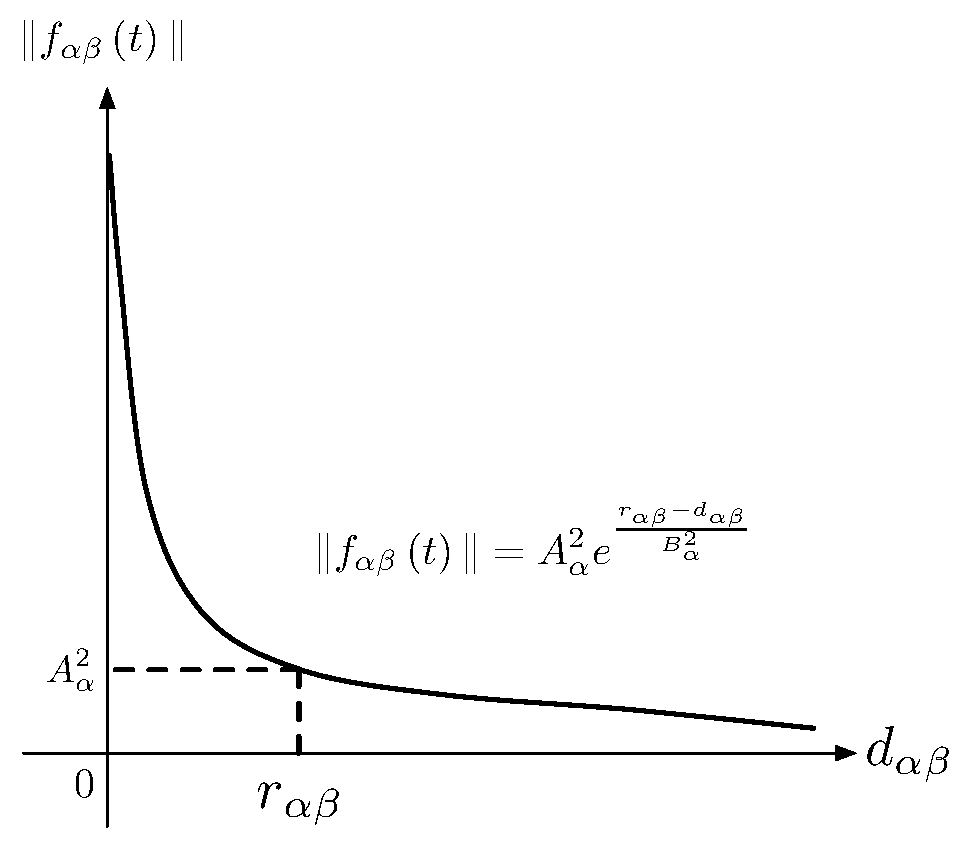
\includegraphics[scale=0.45]{Figures/physicalinteraction.pdf} 
\caption{The function about the interaction force $\vec{f_{\alpha\beta}}(t)$ and the distance between two agents
$d_{\alpha\beta}$ }\label{fig:physicalinteraction}
\end{figure}

There is one intersection of the graph and the axis $ \left( 0, A_{\alpha}^{2} exp\left( \frac{r_{\alpha\beta} }{B_{\alpha}^{2}}\right)  \right)  $. If put into the constants, we will be able to get a maximum value of $ f_{\alpha\beta}(t) $, since the distance between agents cannot be negative. Here we set $ A_{\alpha}^{2} = 3 m/s^{2} $, $ r_{\alpha\beta} = 0.6 m $, and $ B_{\alpha}^{2} = 0.2 m $, so $ f_{\alpha\beta}(t)^{max} \doteq 60 m/s^{2} $, which is about six times the gravitational acceleration and represents a rather large force between agents (as large as six person's weight). \\\\
However, we notice that the effective part of the force calculated above is only the horizontal 
component that enables the agent to move horizontally in the plane where we do the simulation, 
but the reality is that the agents sometimes are also able to move vertically, for example, 
by stepping upon other people when they cannot take the pushing force from the surrounding agents. 
When that happens, the horizontal component of the repulsive force becomes smaller even if 
$d_{\alpha\beta}$ is kept the same.	
Therefore, a qualitative modification of dependence between $ f_{\alpha\beta}(t) $ and $ d_{\alpha\beta} $ could be:
\begin{figure}[hb]   
\centering
    {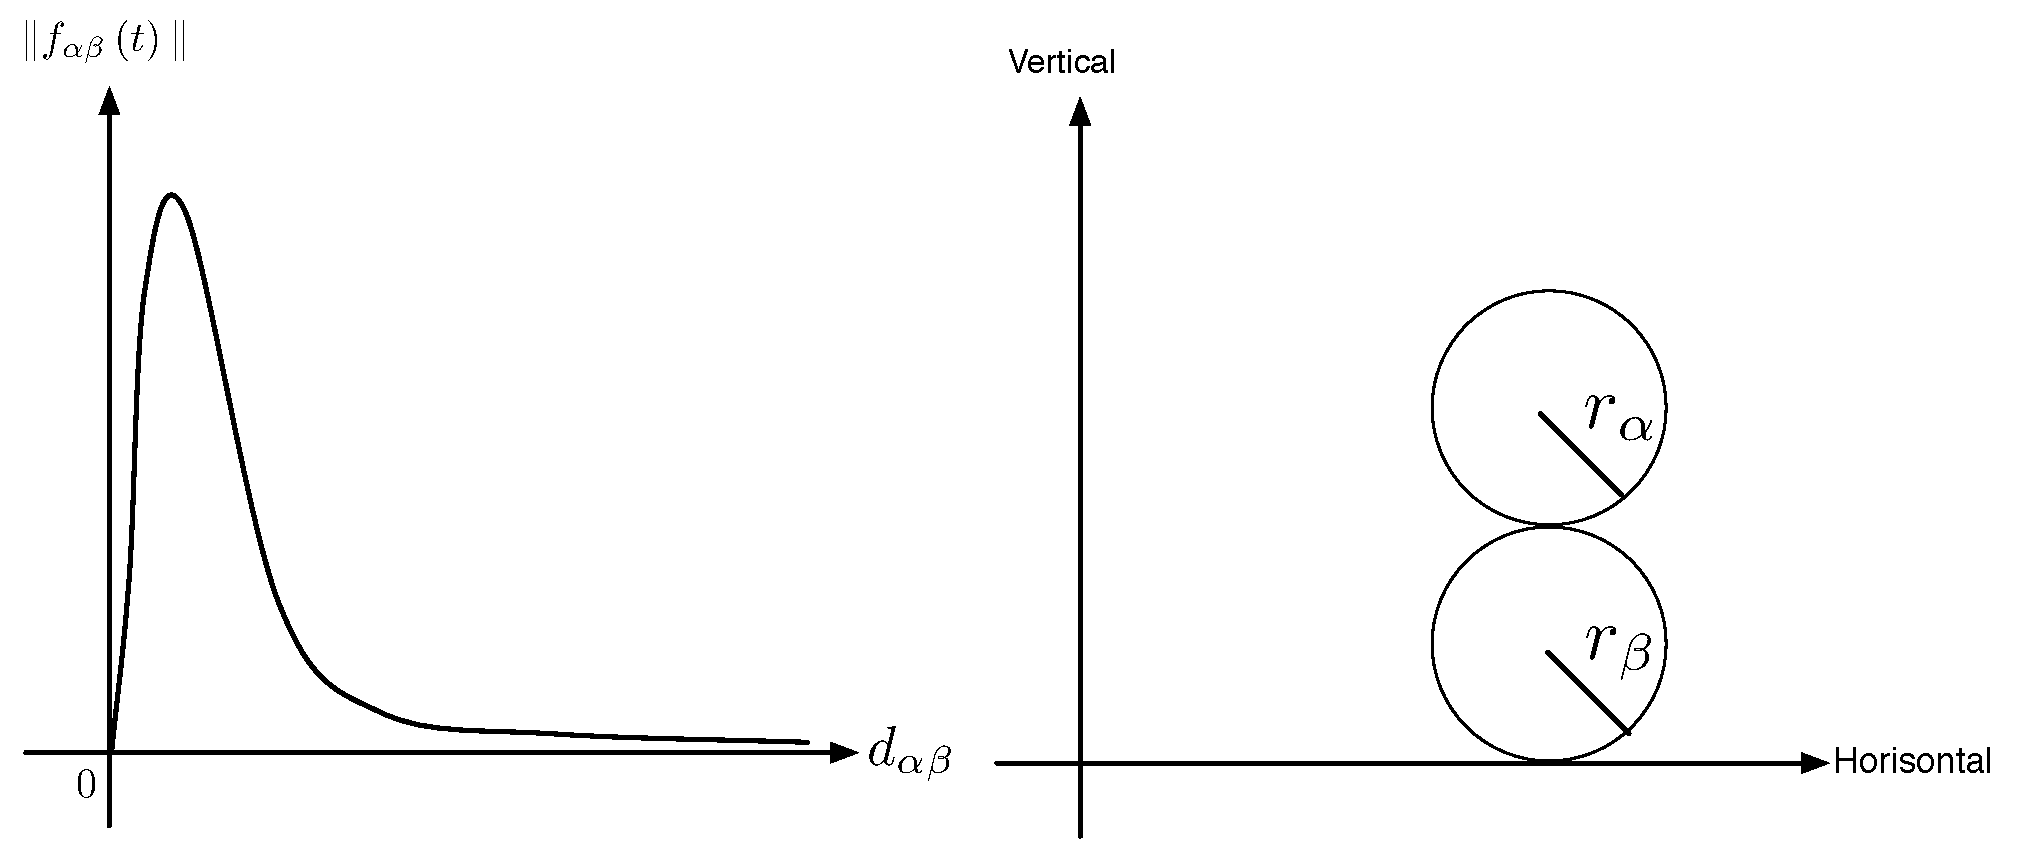
\includegraphics[scale=0.35]{Figures/ForceOverlapping.pdf}} 
    \caption{}
    \label{forceoverlapping}
\end{figure}
\\
\subsection{Use social force in further calculation}
use the value of forces to predict, as they are partly not real forces, the measurement does not reflect the reality in some range.
Pressure
\clearpage
\subsection{characteristics of crowd modeling}
In this section we try to make an outline of what characteristics one could use when
describing a crowd.

%\subsection{The individual}%
%The characteristic of the individual is the following: The individual do not make 
%any complicated decisions, but is approximated to only make very basic decisions.
%
%\begin{itemize}
%\item Desired speed: each individual has a desired walking speed.\\
%\item Actual speed: The individuals speed do not always correspond to the desired speed duel to obstacles and/or other individuals blocking the desired direction.\\
%\item Maximum speed: There is a physical limit to the persons speed.\\
%\item Panic state: The person can panic, resulting in a higher speed and the person no longer respect other persons private space.\\
%\item Impatiens: Depends on the initial conditions.\\
%\item Desired direction: The individual always want to walk towards the exit.\\
%\item Influence from other individuals ($\beta$) on this individual ($\alpha$): Individuals interact and obstruct each other.\\
%\item Influence from walls and/or obsticals on the individual\\
%\item Personal sphere: The individual do'sent want other individuals ($\beta$) to invade his/hers privacy.\\
%\item Attractive forces: For example family, shopping windows etc.\\
%\end{itemize}

The characteristic for the collective group can be divided in to two subcategories: Universal 
characteristic which are the characteristics that are independent of the model used to describe
the situation. Then there are the situation/model specific characteristic. Where the situations specific 
characteristic should arise from simulations of the model, while the universal characteristic 
is used to describe the dynamics of an arbitrary group. 

\subsubsection{Universal characteristic}
A universal characteristic is a characteristic that is independent of the model.

\begin{itemize}
\item Flow rate (pedestrians/time): The number of pedestrians passing a given 
boarder during a given time.
\item Flow rate per. space: Number of pedestrians passing a given boarder during 
a given time, as a function of space. The "space" could be a doorway, with of a
 hall, specific design of a corridor etc.
\item Flow rate/average speed: The number of individuals passing a given boarder pr. 
time as a function of the average speed. (Detect at what speed clocking occurs for example)
\item Density as a function of position (x,y,$\rho$)
\end{itemize}

\subsection{Model specific characteristic}
These characteristic are characteristic which emerge from the model.

\begin{itemize}
\item Each individual is represented by two coupled differential equations representing the position and two coupled differential equations representing the velocity.
\item The initial conditions of the system is determined bye a stochastic spread.
\item At each calculation there will arise an error. The size of this error depends on the size of the time step.
\item A time step which need to be determined optimally.
\item There could be a problem determining if a deviation arise from the error or if it arise because of the stochastic spread. (What viggo said).
\item This model takes a lot of computational power. (I think)
\end{itemize}



\clearpage
% vim:ft=tex
\section{Simulation approach}
\label{sec:simulation}
In this section, we describe how our simulation is implemented, and how the 
implementation works. This is done in part to document our implementation, and 
in part to give the reader an overview of how our results are obtained.
We will describe briefly how the program is structured on a macro level, and 
go into more detail on the parts specific to the calculations of the model 
parameters. The full source code is available online\footnote{See 
\url{http://akira.ruc.dk/~tohojo/crowd-modelling}.}.

Our simulation is implemented in the Python programming language, with the 
calculation intensive parts implemented in C for performance reasons. We 
assume a virtual coordinate system using meters as a base unit, and with the 
origin in the centre of the area we simulate. Each pedestrian is 
described by a centre point and a radius, and each wall is described by a line 
segment connecting two points.

All parameters are stored as double precision floating point values where 
nothing else is indicated. We use custom data structures to keep track of the 
pedestrians and walls while running the simulation. Python is used to set up the 
initial conditions, run the program's main control loop, and draw the 
simulation results through the \emph{PyGame} library \cite{pygame}. This 
allows to do real-time animation as well as saving each simulation step 
to be assembled into a film afterwards. All calculations and data processing 
is done in a Python extension written in C, to increase performance. Gathering 
of data to draw the graphs and the drawing itself is done in the Python code. 

\subsection{Structure of the program}
The program is structured into four main parts: The simulation calculations, 
drawing of the simulations, plotting of parameters and the control part 
setting up parameters and calling the other parts as necessary. The drawing 
part mainly consists of a frontend to the drawing library, and so is not 
interesting to discuss here. The other parts will be described in the 
following, structured so as to present the sequence that is followed when a 
simulation is run. This description consists of three parts: setting up the 
simulation, calculations, and gathering of results.

\subsection{Setting up the simulation}
The program supports defining multiple \emph{scenarios} to simulate. Each 
scenario defines its own set of parameters, and a simulation run features one 
scenario. The parameters defined for each scenario include:

\begin{itemize*}
    \item The model constants, $A$, $B$, $U$, $\lambda$ and pedestrian relaxation 
        time. These are the same for all pedestrians in a simulation.
    \item Mean initial desired velocity and radius of pedestrians and their standard 
        deviation, and the factor used to calculate the maximum velocity.
    \item The initial number of pedestrians, the area(s) they start in and the 
        target(s) they move towards.
    \item The geometry of the scenario (i.e. placement of walls).
    \item Definition of the areas where measurement of data for plotting 
        graphs is done and which parameters should be plotted (see 
        section~\ref{sec:measurement}).
    \item Various parameters related to drawing of the simulation, maximum run 
        time and optional continuous inflow of pedestrians.
\end{itemize*}

Parameters that are not set for each scenario, but are defined once for all 
simulations are:

\begin{itemize*}
    \item Time step size.
    \item Plotting data sampling frequency.
\end{itemize*}

How the values of the parameters are determined is described in 
section~\ref{sec:init-cond}. From these parameters, the simulation is set up 
by initialising the calculation module and creating the pedestrians.

The pedestrians are created with an initial velocity of zero, and distributed 
randomly within the area(s) designated by the parameters for the scenario, as 
described in section~\ref{sec:init-pedestrians}. 

\subsection{Calculation of the model}
\label{sec:model-calculation}
For each step of the simulation, the calculations are run in two parts: 
Finding the accelerations (or resulting force) for all pedestrians, and 
updating position and velocity for the pedestrians.  Since the acceleration 
for each pedestrian is dependent on both position and velocity of the other 
pedestrians, splitting the calculations this way enables us to do the 
calculations of pedestrians in any order, and even parallel. The drawback 
is that the pedestrians are only affected by the movement and positions of 
other pedestrians as they were at the end of the last simulation step. This 
means that the time step has to be small enough that this doesn't matter in 
practice.

The acceleration vectors for each pedestrian, $\alpha$, is calculated in three 
steps, corresponding to the parts $\overrightarrow{f_\alpha^d}$, 
$\overrightarrow{f_{\alpha \beta}}$ and $\overrightarrow{f_{\alpha \gamma}}$ from 
section~\ref{sec:the-model}. In each simulation step the three forces are 
calculated in order, first calculating the desired force, then the repulsive 
force from each of the other pedestrians in the simulation, and finally the 
repulsive force from each wall. The resulting vectors are added to yield the 
total acceleration for each pedestrian.

After this is calculated for all pedestrians, their velocities and positions are 
updated in separate steps. Each of these four steps are described in detail 
in the following. The code calling the other parts of the calculation can be 
seen in code segment~\ref{lst:calling}. This function is called once for each 
pedestrian (index \texttt{i}) for each simulation step.

\begin{lstlisting}[caption={Main function calling the other parts of the 
    calculation code.},label=lst:calling]
void calculate_forces(Py_ssize_t i)
{
    int j;
    add_desired_acceleration(&pedestrians[i]);

    for(j = 0; j < a_count; j++) {
        if(i == j) continue;
        add_repulsion(&pedestrians[i], &pedestrians[j]);
    }

    add_wall_repulsion(&pedestrians[i]);
}
\end{lstlisting}

\subsubsection{Calculating the desired force}
The function for calculating the desired force can be seen in code 
segment~\ref{lst:desired-force}. Of note is the implementation on lines 7-19 
of the conditional definition of $V_\alpha^d(t)$ given in 
equation~\eqref{eqn:cond-define} and the creation of a unit vector in lines 
20-21 to add the direction to the desired velocity.

To increase performance, it is preferred to update values in place, instead of 
copying them around in different parts of the computer's memory. This gives 
rise to the constructs around the \texttt{vector\_i*}-functions in the code; 
here the \emph{i} stands for ``in place''.

\begin{lstlisting}[caption={Calculating the desired 
    force.},label=lst:desired-force]
static void add_desired_acceleration(Pedestrian * a)
{
    double average_velocity = 0.0, impatience = 0.0, 
           desired_velocity = 0.0;
    Vector desired_direction = {0.0, 0.0};

    if(a->time) {
        double proj = vector_projection_length(
                a->initial_position, a->target, a->position);
        average_velocity = proj / a->time;

        impatience = 1.0 - average_velocity / a->initial_desired_velocity;

        desired_velocity = (1.0-impatience) * a->initial_desired_velocity + \
                           impatience * a->max_velocity;

    } else {
        desired_velocity = a->initial_desired_velocity;
    }
    desired_direction = vector_sub(a->target, a->position);
    vector_unitise(&desired_direction);

    a->acceleration = vector_mul(desired_direction, desired_velocity);
    vector_isub(&a->acceleration, &a->velocity);
    vector_imul(&a->acceleration, 1.0/a->relax_time);
}
\end{lstlisting}

\subsubsection{Repulsion from other pedestrians}
The two functions used for calculating the repulsion from other pedestrians is seen 
in code segment~\ref{lst:pedestrian-repulsion}. The \texttt{add\_repulsion} function 
is called for each pair of pedestrians. The force without any angle dependence is 
calculated in the \texttt{calculate\_repulsion} function, and is modified by 
the angular dependence if the pedestrian's velocity is not zero, and $\lambda$ is 
not one. If the velocity is zero, calculating the dot product would result in 
a division by zero, and if $\lambda$ is one, modifying the force by the 
angular dependence would have no effect. The whole calculation is skipped if 
one of the constants $A$ or $B$ are zero, as this would make the calculations 
have no effect, or result in a division by zero, respectively.

\begin{lstlisting}[caption={Calculating the repulsion from other 
    pedestrians.},label=lst:pedestrian-repulsion]
Vector calculate_repulsion(Pedestrian * a, Pedestrian * b, double A, double B)
{
    double radius_sum = a->radius + b->radius;
    Vector from_b     = vector_sub(a->position, b->position);
    double distance   = vector_length(from_b);

    vector_unitise(&from_b);
    vector_imul(&from_b, A * exp((radius_sum-distance)/B));

    return from_b;
}

void add_repulsion(Pedestrian * a, Pedestrian * b)
{
    if(!A || !B) return;
    Vector repulsion = calculate_repulsion(a, b, A, B);
	if(a->velocity.x && a->velocity.y && lambda < 1.0) {
		Vector from_a = vector_sub(b->position, a->position);

		double cosine = vector_dot(a->velocity, from_a)/(
				vector_length(a->velocity) * vector_length(from_a));

		vector_imul(&repulsion, (lambda + (1-lambda)*((1+cosine)/2)));
	}
    vector_iadd(&a->acceleration, &repulsion);
}
\end{lstlisting}

\subsubsection{Repulsion from walls}
The code for adding the repulsion from the walls is shown in code 
segment~\ref{lst:wall-repulsion}. The \texttt{add\_wall\_repulsion} function 
is called for each pedestrian and consists of two parts: Finding the points on the 
walls where repulsion should be calculated from, and calculating the repulsion 
from these points. The force from the repulsion points is calculated in the 
function \texttt{calculate\_wall\_repulsion} that is called for each repulsion 
point. This calculation corresponds to equation~\eqref{eqn:wall-repulsion}.

\begin{lstlisting}[caption={Calculating the repulsion from the 
    walls.},label=lst:wall-repulsion]
void add_wall_repulsion(Pedestrian * a)
{
    int i;
    Vector * repulsion_points  = PyMem_Malloc(w_count * sizeof(Vector));
    int rep_p_c = 0;
    Vector repulsion;

    rep_p_c = find_repulsion_points(a, repulsion_points);

    for(i = 0; i < rep_p_c; i++) {
        repulsion = calculate_wall_repulsion(a, repulsion_points[i]);
        vector_iadd(&a->acceleration, &repulsion);
    }


    PyMem_Free(repulsion_points);
}

Vector calculate_wall_repulsion(Pedestrian * a, Vector repulsion_point)
{
    Vector repulsion_vector = vector_sub(a->position, repulsion_point);
    double repulsion_length = vector_length(repulsion_vector);
    vector_unitise_c(&repulsion_vector, repulsion_length);

    double repulsion_force = (1/a->radius) * U * exp(-repulsion_length/a->radius);

    vector_imul(&repulsion_vector, repulsion_force);

    return repulsion_vector;
}
\end{lstlisting}

The function for finding the repulsion points on the walls is seen in code 
segment~\ref{lst:repulsion-points}. This is an implementation of the algorithm 
described in section~\ref{sec:repulsion-points}. Lines 9-27 corresponds to 
step one in the algorithm description that identifies definite repulsion 
points (those that are not wall endpoints) and possible repulsion points 
(those that are endpoints).

In lines 29-35 an endpoint is discarded if it is already used because it is 
shared with a wall that has already defined a repulsion point. In lines 36-57 
endpoints that are not discarded in this way are added to the list of 
repulsion points if they are either not free-floating (i.e. shared with 
another wall), or closer to the pedestrian centre than the pedestrian's 
radius. This ensures that doorways do not repulse pedestrians that are passing 
through it.

\begin{lstlisting}[caption={Finding the wall repulsion 
    points.},label=lst:repulsion-points]
int find_repulsion_points(Pedestrian * a, Vector repulsion_points[])
{
    int i,j;
    double projection_length;
    Vector * used_endpoints     = PyMem_Malloc(2*w_count * sizeof(Vector));
    Vector * possible_endpoints = PyMem_Malloc(w_count * sizeof(Vector));
    int rep_p_c = 0, use_e_c = 0, pos_e_c = 0;

    for(i = 0; i < w_count; i++) {
        Wall w = walls[i];
        projection_length = vector_projection_length(w.start, w.end, a->position);
        if(projection_length < 0)  {
            possible_endpoints[pos_e_c++] = w.start;
        } else if(projection_length > w.length) {
            possible_endpoints[pos_e_c++] = w.end;
        } else {
            // We have the length, L, of how far along AB the projection point is.
            // To turn this into a point, we multiply AB with L/|AB| and add
            // this vector to the starting point A.
			// P = A + AB*L/|AB|
            repulsion_points[rep_p_c++] = vector_add(w.start, 
                    vector_mul(vector_sub(w.end, w.start), 
                        projection_length/w.length));
            used_endpoints[use_e_c++] = w.start;
            used_endpoints[use_e_c++] = w.end;
        }
    }

    for(i = 0; i < pos_e_c; i++) {
        int use_e = 1;
        for(j = 0; j < use_e_c; j++) {
            if(vector_equals(possible_endpoints[i], used_endpoints[j])) {
                use_e = 0;
            }
        }
        if(use_e) {
			// Keep track of whether the endpoint is free-floating, i.e. if
			// it is shared with another wall.
			int free_e = 1;
			for(j = 0; j < pos_e_c; j++) {
				if(i != j && 
						vector_equals(possible_endpoints[i],
							possible_endpoints[j])) {
					free_e = 0;
				}
			}
			// Endpoints that are free-floating (i.e. sides of doorways) are
			// only considered for repulsion if they are closer to the pedestrian
			// than the pedestrian's radius. This allows pedestrians to pass more
			// freely through doorways.
			if(!free_e || 
					vector_length(vector_sub(a->position,
							possible_endpoints[i])) < a->radius) {
				repulsion_points[rep_p_c++] = possible_endpoints[i];
				used_endpoints[use_e_c++] = possible_endpoints[i];
			}
        }
    }

    PyMem_Free(used_endpoints);
    PyMem_Free(possible_endpoints);

    return rep_p_c;
}
\end{lstlisting}

\subsubsection{Updating position and velocity}
After every pedestrian has been updated with a resulting acceleration vector from 
the current simulation step, all pedestrians update their position and velocity.  
The position is updated by calculating a displacement vector as explained in 
section~\ref{sec:continuous-movement}.

After updating the position, the pedestrian's velocity is updated by adding 
the acceleration vector, to be used for the next simulation step. The code 
that does this is seen in code segment~\ref{lst:update-position}. Line 14 is 
related to the measuring of data for plotting, and will be explained in 
section~\ref{sec:measurement}.

\begin{lstlisting}[caption={Updating the pedestrian 
    position.},label=lst:update-position]
void update_position(Pedestrian * a)
{
	Vector delta_p = vector_add(
			vector_mul(a->velocity, timestep), 
			vector_mul(a->acceleration, 0.5 * pow(timestep, 2)));

    vector_iadd(&a->position, &delta_p);
	a->velocity = vector_add(a->velocity,
			vector_mul(a->acceleration, timestep));
    a->time += timestep;

    check_flowlines(a);
}
\end{lstlisting}

\subsection{Obtaining results}
\label{sec:measurement}
There are two ways we obtain results from the simulation: through the drawings 
of the simulations themselves, and through graphs of various measurements made 
during the simulation. In this section we describe the mechanisms for 
obtaining these results. Which results are used for which scenarios are 
described, along with the scenarios themselves, in section~\ref{sec:results}.

\subsubsection{Drawings of the simulation}
When the simulation is run, drawings of the pedestrian's positions, walls etc. are 
created for each simulation step. These can be shown in real time, or saved 
and either assembled into a film or used as individual illustrations. We use 
these images to make qualitative assessments of pedestrian behaviour, e.g. 
determining whether a lane formation occurs. We include the relevant images as 
illustrations in the results section.

\subsubsection{Graphs of measurements}
As part of the simulation program, we have added measurements of various 
properties of the simulation, which are then assembled into graphs after the 
simulation has run. This section describes the measuring features we have 
added to the program, and \emph{how} they work. \emph{Why} we measure each 
property is explained along with the results. Since we have revised which 
graphs are needed throughout our work with the simulations, some additional 
measuring and graphing features exist in the source code, but are not 
described here.

The graphing functionality works in two different modes: One is graphing 
properties as a function of the simulation time, and others run multiple 
simulations varying one or more parameters and graphing properties as a 
function of this varied parameter. Any numeric parameter can be varied in this 
way. It is noted for each feature in which mode it is used and some properties 
are used for both modes. The properties we measure are:

% TODO: Pros and cons of these measurements.

\begin{itemize}

    \item \textbf{Flow rate:} Flow rate is measured along a line segment 
        defined as a parameter to the scenario; the line segment is assumed to 
        be perpendicular to the primary movement direction of the pedestrians.  
        The simulation keeps track of at what time each pedestrian first comes 
        into contact with this line segment, i.e. is first less than their 
        radius away from it . This is used as an approximation of when the 
        pedestrians cross the line. The average flow rate is then computed as 
        the number of pedestrians who have crossed the line divided by the 
        time.  This is graphed as a function of time, using a five second 
        moving average, and as a function of parameters, using the average of 
        the flow rate measurements of an entire simulation.

    \item \textbf{Leaving time:} The leaving time is a measure of how long it 
        takes for all pedestrians to leave the simulation completely. Pedestrians are 
        removed from the simulation when they reach their target, or when they 
        get outside the calculation area which is the basis of this 
        measurement. This property is only measured for a whole simulation, 
        and as such is only graphed as a function of the varying parameters. 
        Of course simulations that do not have a finite running time (i.e. 
        where pedestrians are added continuously, or where they never reach their 
        target) do not measure this property.
\end{itemize}

\subsection{Summary}
In this section we have described our implementation of the simulation. The 
program is split up into three parts: setting up the simulation with 
parameters and initial conditions, the calculations of the model itself, and 
measurements of the results. The first and last parts are implemented in the 
Python programming language, while the calculations themselves are implemented 
in C for performance reasons. The measurements of simulation results include 
drawing of pictures of the simulation, and graphs of the flow rate and the 
time it takes all pedestrians to leave a room.

\clearpage
\section{Result}
a
\clearpage
\section{Perspective}
a
\clearpage
\section{Conclusion}
a
\clearpage
% vim:ft=tex
\section{Appendix}
\section{calculation}
In this simplified situation, there is no wall and only one other pedestrian $\beta$ at position $(-\frac{\sqrt{2}}{5}, \frac{\sqrt{2}}{5})$ which exert expelling force to $\alpha$.  The exit is reduced to one point $E(4,4)$.  Their positions at $t=0$ is shown in the drawing below:\\

\begin{figure}
\centering
{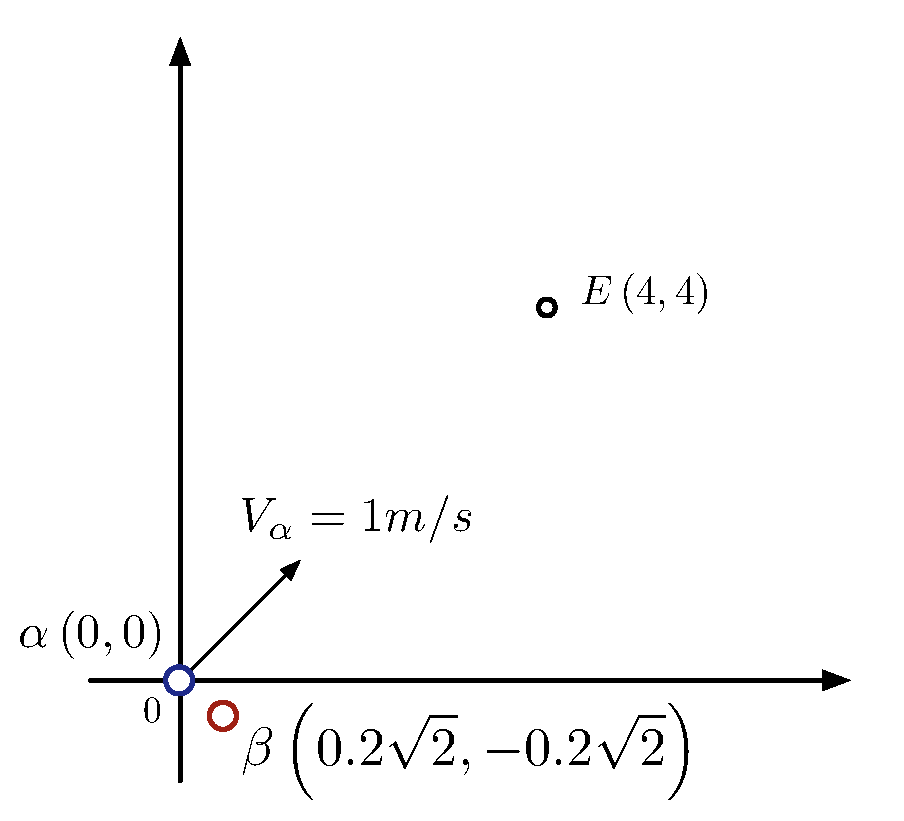
\includegraphics[scale=0.45]{calculation.pdf}} 
\caption{\small{}\label{calc}}
\end{figure}

In addition, to complete the initial conditions, we need to know $\alpha$'s actual velocity at $t=0$, suppose $\overrightarrow{v_{\alpha}(0)}=(\frac{\sqrt{2}}{2}, \frac{\sqrt{2}}{2})$, also the average speed into the desired direction of motion $\overline{v_{\alpha}(0)}=0$.\\

With those numbers we can calculate the impatience factor 
 \begin{equation}
 n_{\alpha}(0)=1-\frac{\overline{v_{\alpha}(0)}}{v^{0}_{\alpha}(0)}=1-\dfrac{0}{v^{0}_{\alpha}(0)}=1
 \end{equation}

so 
 \begin{equation}
 v^{0}_{\alpha}(0)=[1-n_{\alpha}(0)]v^{0}_{\alpha}(0) + n_{\alpha}(0)v_{\alpha}^{max} = v_{\alpha}^{max}
 \end{equation}
 
Suppose $v_{\alpha}^{max}=3$, then 

 \begin{equation}
 	\vec{f^{0}_{\alpha}} \left( \vec{v_{\alpha}} \right) 
= 	\frac{1}{\tau_{\alpha}} \left( v^{0}_{\alpha} 
	\vec{e_{\alpha}} - \vec{v_{\alpha}} \right)
 \end{equation}
 
where $\tau_{\alpha}=1$,
 \begin{equation}
 \overrightarrow{f^{0}_{\alpha}}\overrightarrow{v_{\alpha}} = (\sqrt{2}, \sqrt{2})
 \end{equation}

Another part of $\alpha$'s acceleration is from the repelling force from $\beta$, in order to speed  up the calculation here we omit the not so important part in calculating $\overrightarrow{f_{\alpha \beta}}$.
Therefore,
 \begin{equation}
 \overrightarrow{f_{\alpha \beta}} = A^{2}_{\alpha} exp(\frac{r_{\alpha\beta}-d_{\alpha\beta}}{B^{2}_{\alpha}})\overrightarrow{n_{\alpha \beta}}
 \end{equation}
where $A^{2}_{\alpha}=3, B^{2}_{\alpha}=0.2, r_{\alpha\beta}=0.6, d_{\alpha\beta}=0.4$, and $\overrightarrow{n_{\alpha \beta}}=(-\frac{\sqrt{2}}{2}, \frac{\sqrt{2}}{2})$,
so 
 \begin{equation}
 \overrightarrow{f_{\alpha \beta}} = 8(-\frac{\sqrt{2}}{2}, \frac{\sqrt{2}}{2})
 \end{equation}
In all, the acceleration of $\alpha$ is 
 \begin{equation}
 \overrightarrow{f_{\alpha}(0)} = \overrightarrow{f^{0}_{\alpha}}\overrightarrow{v_{\alpha}} + \overrightarrow{f_{\alpha\beta}} = (-3\sqrt{2}, 5\sqrt{2})
 \end{equation}
Now we are ready to calculate where $\alpha$ is after $\bigtriangleup t=0.1$, if we assume $\alpha$ moves with a constant acceleration during that small time interval.
As the motion is in two dimensions, we need to calculate the displacement in $x$ and $y$ axis respectively.

 \begin{equation}
 r^{x}_{\alpha} = v^{x}_{\alpha} \bigtriangleup t + \frac{1}{2} f^{x}_{\alpha} \bigtriangleup t ^{2}
 \end{equation}
 
 For the y direction,
  \begin{equation}
 r^{y}_{\alpha} = v^{y}_{\alpha} \bigtriangleup t + \frac{1}{2} f^{y}_{\alpha} \bigtriangleup t ^{2}
 \end{equation}
 Therefore, $r_{\alpha}(0.1)= (0.05, 0.1)$
\subsection{Table of notation}
\begin{center}
\begin{tabular}{lll}
\hline
\multicolumn{3}{|c|}{\emph{List of constants and variables}}\\
\hline
\small{\textbf{Symbol}} & \small{\textbf{Description}} & \small{\textbf{Unit}}\\
\hline
$A_{\alpha}^{1}$ & \small{Controls the strength of the personal space force}\\
\hline
$A_{\alpha}^{2}$ & \small{Controls the strength of physical collisions}  & \\
\hline
$B_{\alpha}^{1}$ & \small{Controls the range of the personal space force} & \\
\hline
$B_{\alpha}^{2}$ & \small{Controls the range of physical collisions} & \\
\hline
$\lambda_{\alpha}$ & The anisotropic character of pedestrian interaction & \\
\hline
$\vec{f_{\alpha}} \left( t \right)$ & All forces acting on pedestrian $\alpha$  & \\
\hline
$\vec{f_{\alpha B}} \left( \vec{r_{\alpha}} \right)$ & Force on pedestrian $\alpha$ from walls & \\
\hline
$\vec{f_{\alpha \beta}} \left( \vec{r_{\alpha}}, \vec{r_{\beta}}, \vec{V_{\alpha}}, \vec{V_{\beta}} \right)$ & Force on pedestrian $\alpha$ from pedestrian $\beta$ & \\
\hline
$\vec{f_{\alpha i}} \left( \vec{r_{\alpha}}, \vec{r_{i}}, t \right)$ & Force on pedestrian $\alpha$ from attractions & \\
\hline
$V_{\alpha}^{0}$ & Initial speed of pedestrian $\alpha$ & \\
\hline
$V_{\alpha}^{\text{max}}$ & Maximum speed of pedestrian $\alpha$ & \\
\hline
$\vec{V_{\alpha}^{\text{0}}}$ & Desired velocity of pedestrian $\alpha$ & \\
\hline
$\overline{V}_{\alpha}$ & Average speed in desired direction & \\
\hline
$\vec{e}_{\alpha}$ & Vector pointing in desired direction of pedestrian $\alpha$ & \\
\hline
$\vec{r}_{\alpha}\left( t \right) $ & Vector pointing to position of pedestrian $\alpha$ at time t & \\
\hline
$\vec{r}_{B}$ & Vector pointing to nearest point of wall & \\
\hline
$r_{\alpha}$ & Radius of pedestrian $\alpha$ & \\
\hline
$r_{\beta}$ & Radius of pedestrian $\beta$ & \\
\hline
$r_{\alpha \beta}$ & The sum of the radii of pedestrian $\alpha$ and $\beta$ & \\
\hline
$\vec{X}_{\alpha}$ & Vector pointing to center of mass of pedestrian $\alpha$ & \\
\hline
$\vec{X}_{\beta}$ & Vector pointing to center of mass of pedestrian $\beta$ & \\
\hline
$d_{\alpha \beta}$ & Distance between center of mass of pedestrian $\alpha$ and $\beta$ & \\
\hline
$\tau_{\alpha}$ & Relaxation time $\alpha$ and $\beta$ & \\
\hline
$\eta_{\alpha}$ & Impatience of pedestrian $\alpha$ at time t & \\
\hline
$\vec{\eta}_{\alpha \beta}\left( t \right)$ & Normal vector pointing from $\alpha$ to $\beta$ at time t & \\
\hline
$\vec{\xi}\left( t \right)$ & Stochastic element & \\
\hline
$\phi_{\alpha \beta} \left( t \right)$ & Angle between pedestrian $\alpha$ and $\beta$ & \\
\hline
\label{tableofconstandvar}
\end{tabular}
\end{center}
\clearpage
\bibliographystyle{ruc}
\bibliography{crowd-modelling}
\clearpage

\end{document}
